\cleardoublepage
{
\chapternonum{附录}

\appendixsecmajornumbering

\section{更多SCV检测算法的典型案例}

\autoref{fig:detect_details2}给出了更多应用SCV算法进行波形检测的案例。可以看到,在大多数场景里SCV算法有着优异的检测性能。但对某些数据的处理仍有提高空间,如\autoref{fig:c_xjh}中在$6.5s$处有较为明显的检测错误。
\begin{figure}[htbp]
    \centering
    \subfigure[\label{fig:c_by}被试BY的波形检测结果(局部)]{
    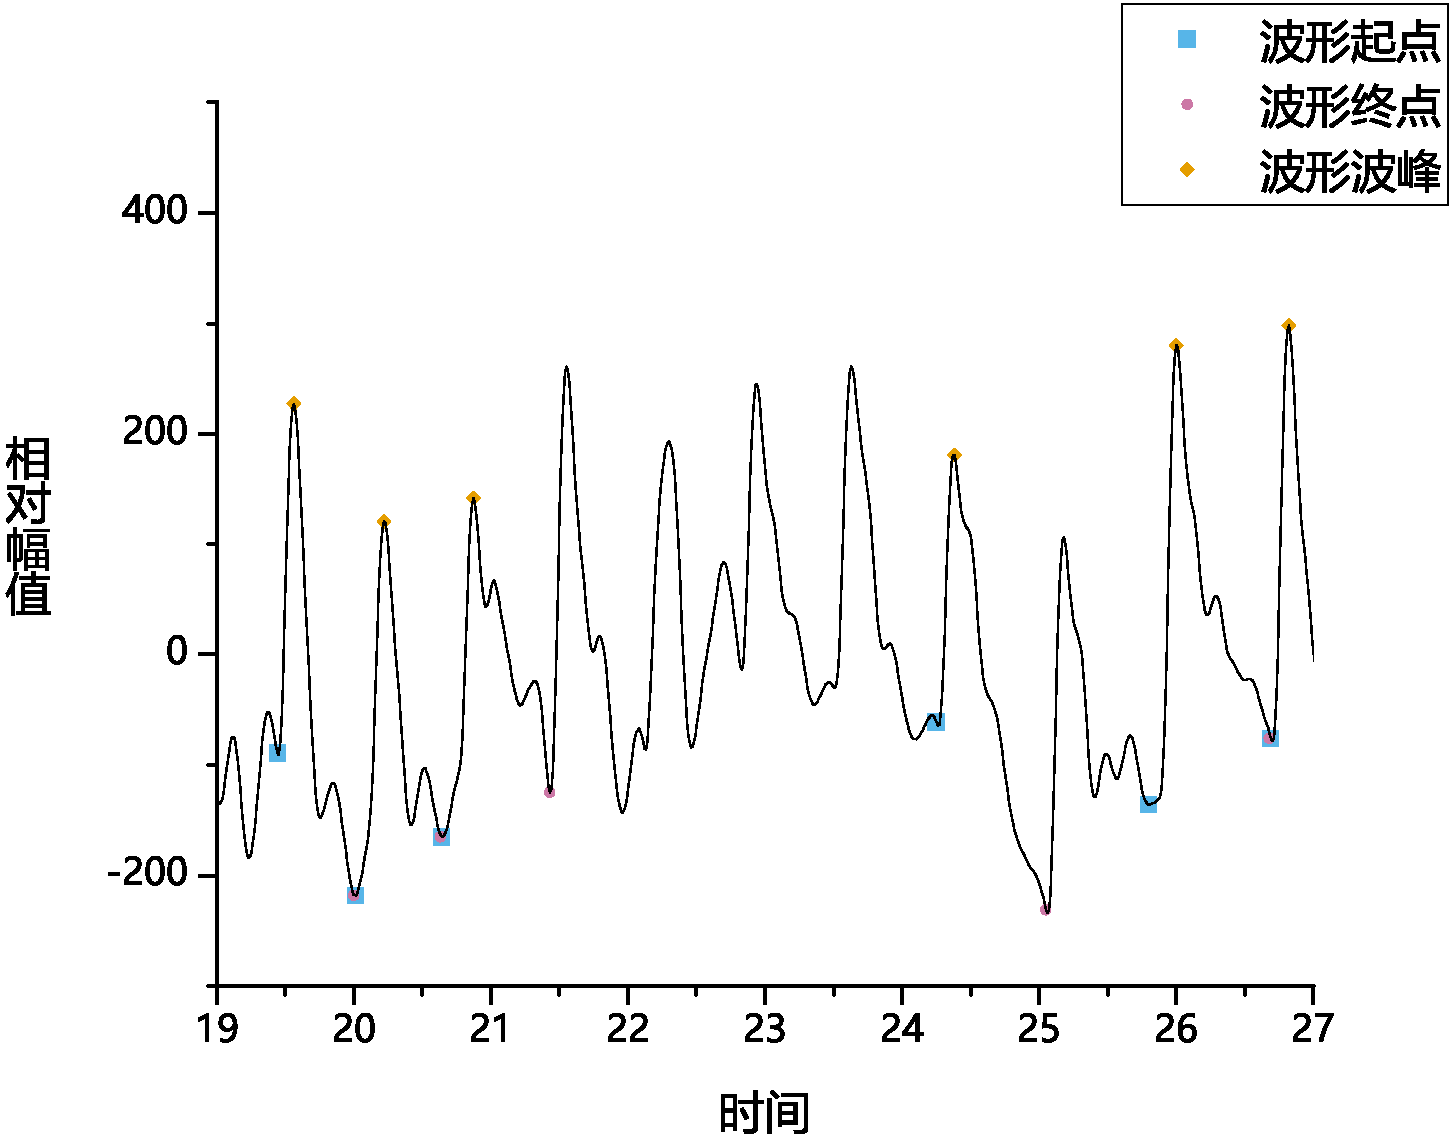
\includegraphics[width=7.5cm]{pulse_preprocess/check/by}
    }
    \quad
    \subfigure[\label{fig:c_ljj}被试LJJ的波形检测结果(局部)]{
    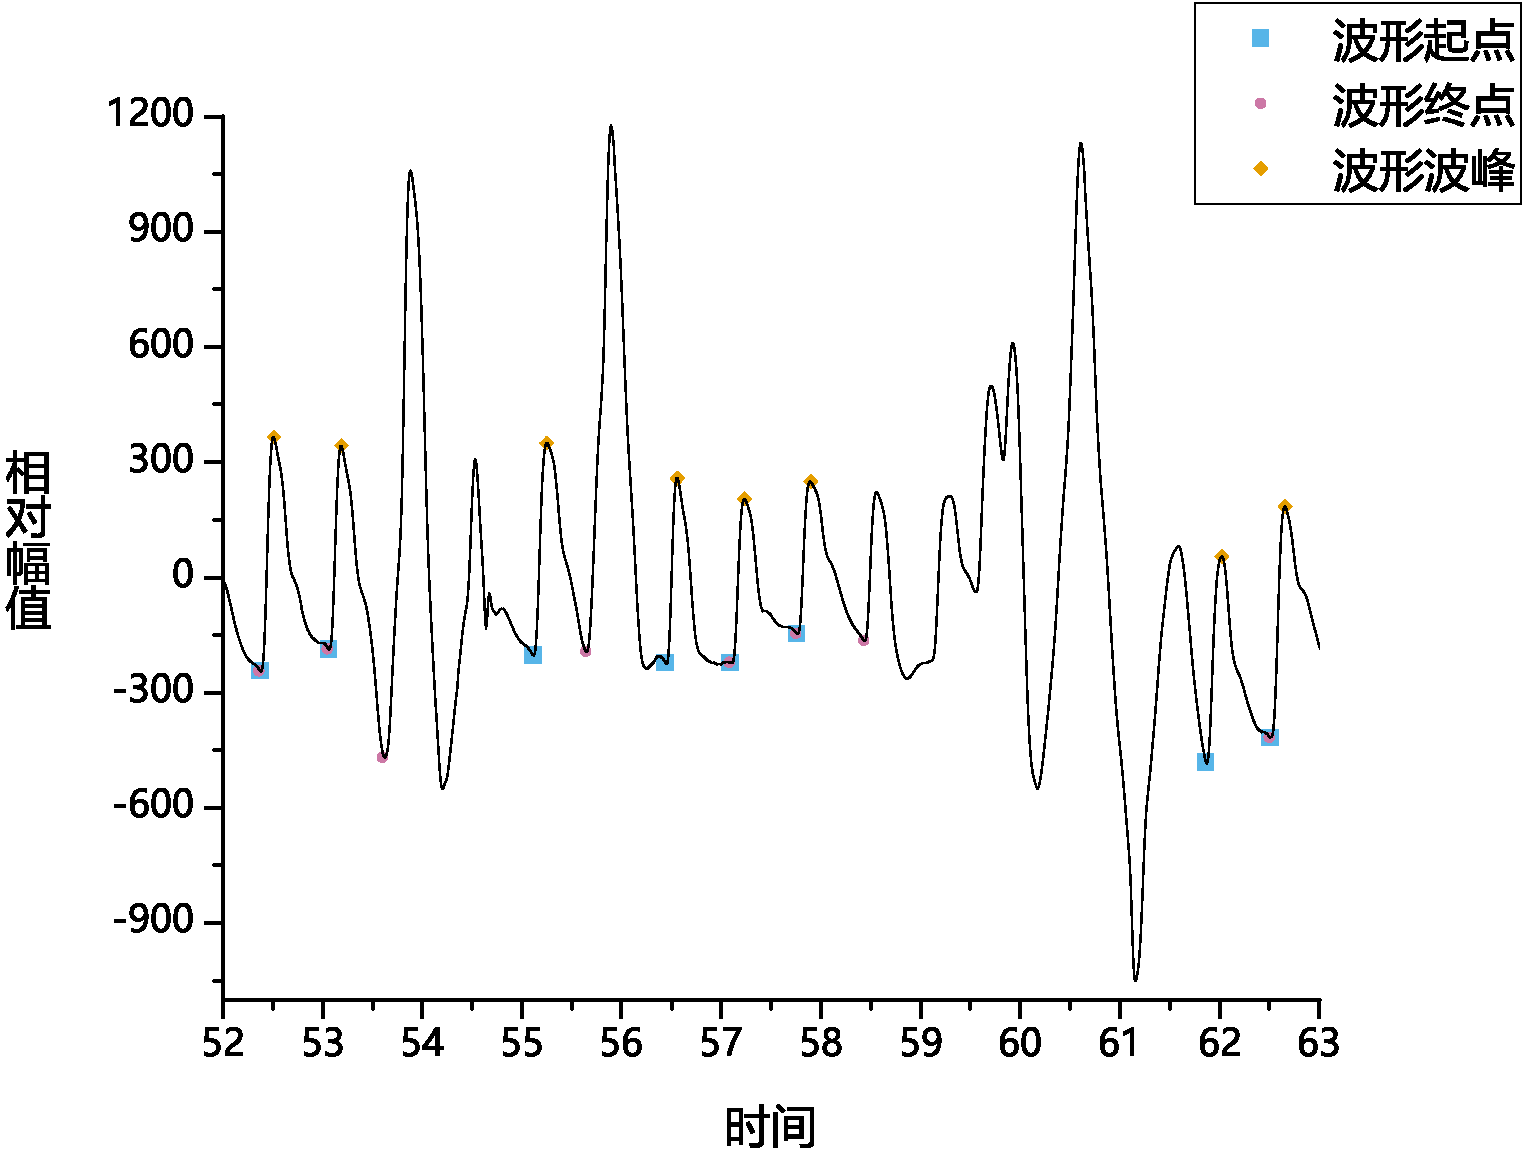
\includegraphics[width=7.5cm]{pulse_preprocess/check/ljj}
    }
    \quad
    \subfigure[\label{fig:c_rmq}被试RMQ的波形检测结果(局部)]{
        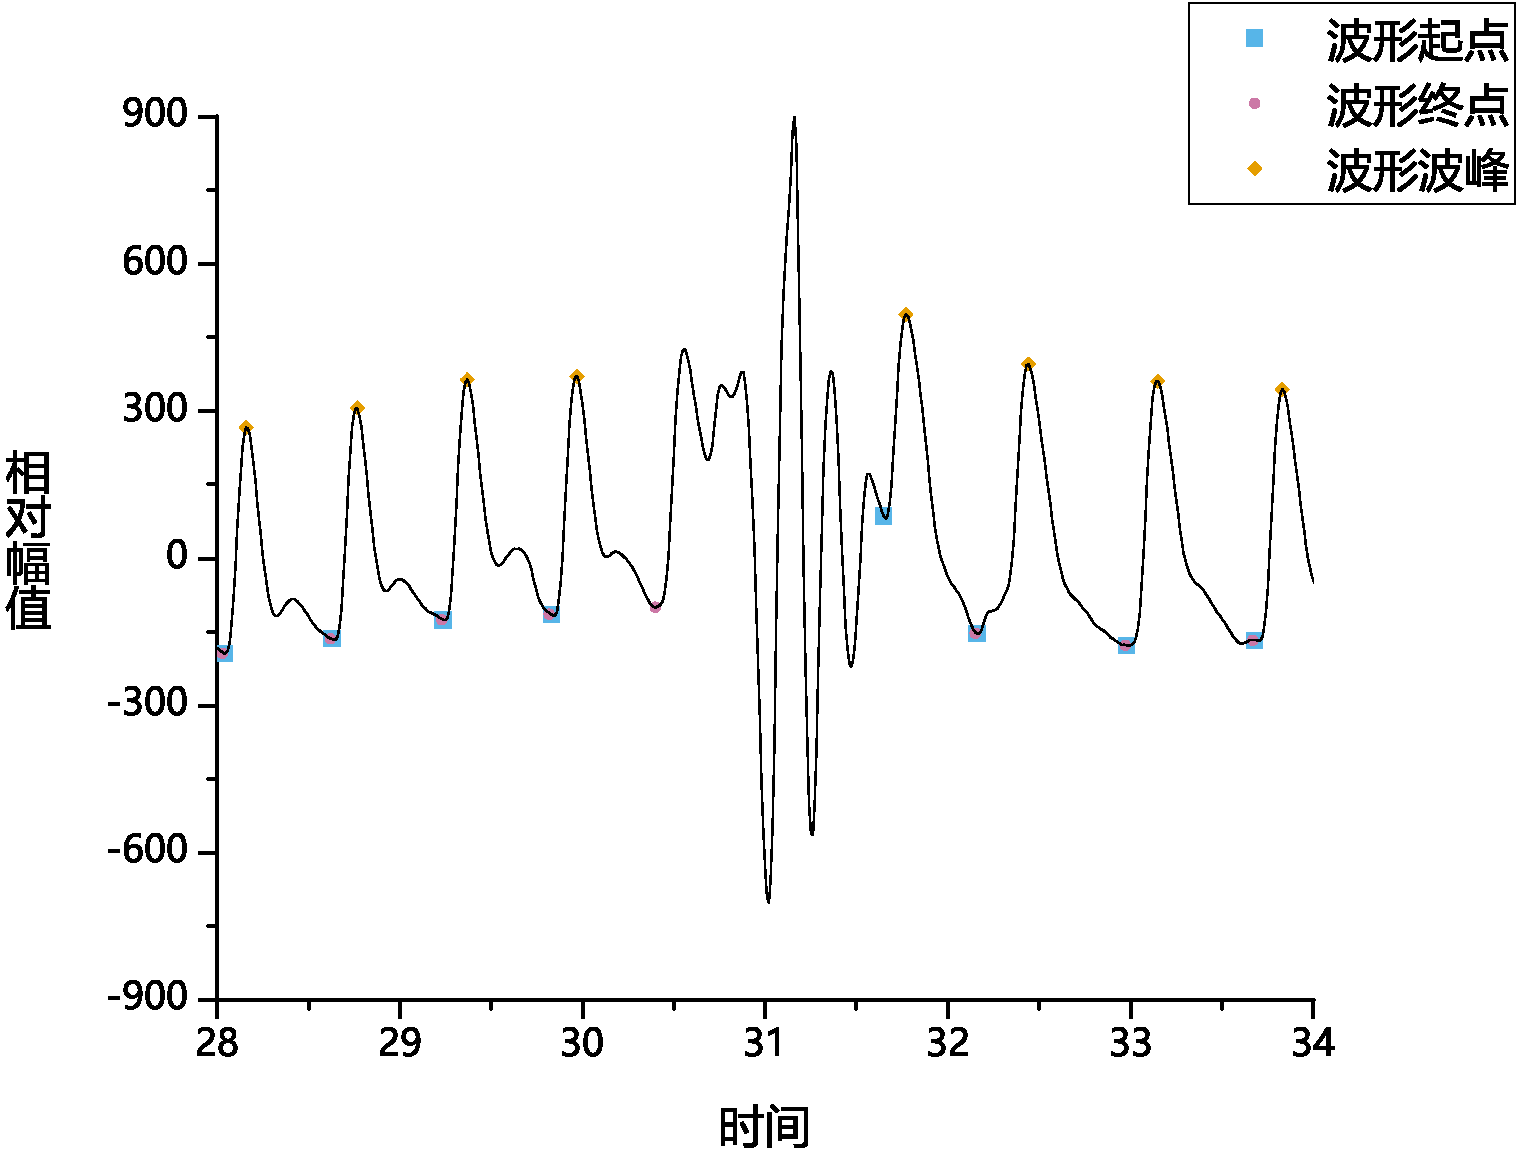
\includegraphics[width=7.5cm]{pulse_preprocess/check/rmq}
    }
    \quad
    \subfigure[\label{fig:c_wc}被试WC的波形检测结果(局部)]{
        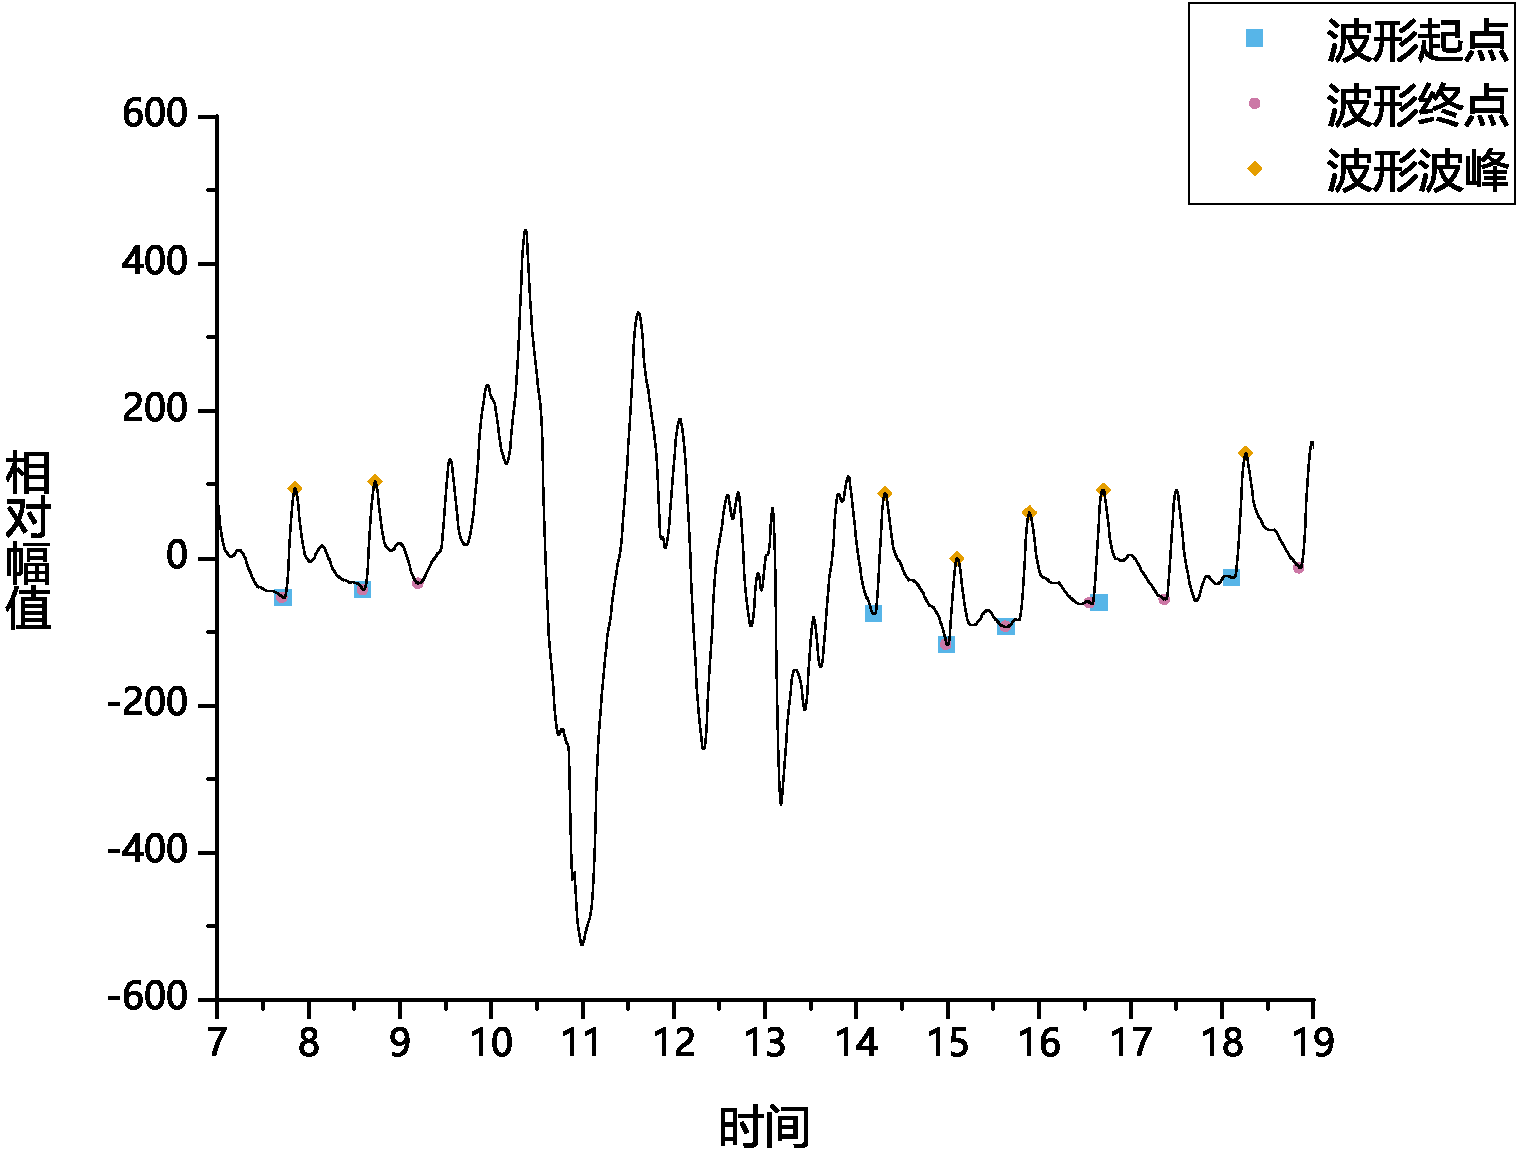
\includegraphics[width=7.5cm]{pulse_preprocess/check/wc2}
    }
    \quad
    \subfigure[\label{fig:c_why}被试WHY的波形检测结果(局部)]{
        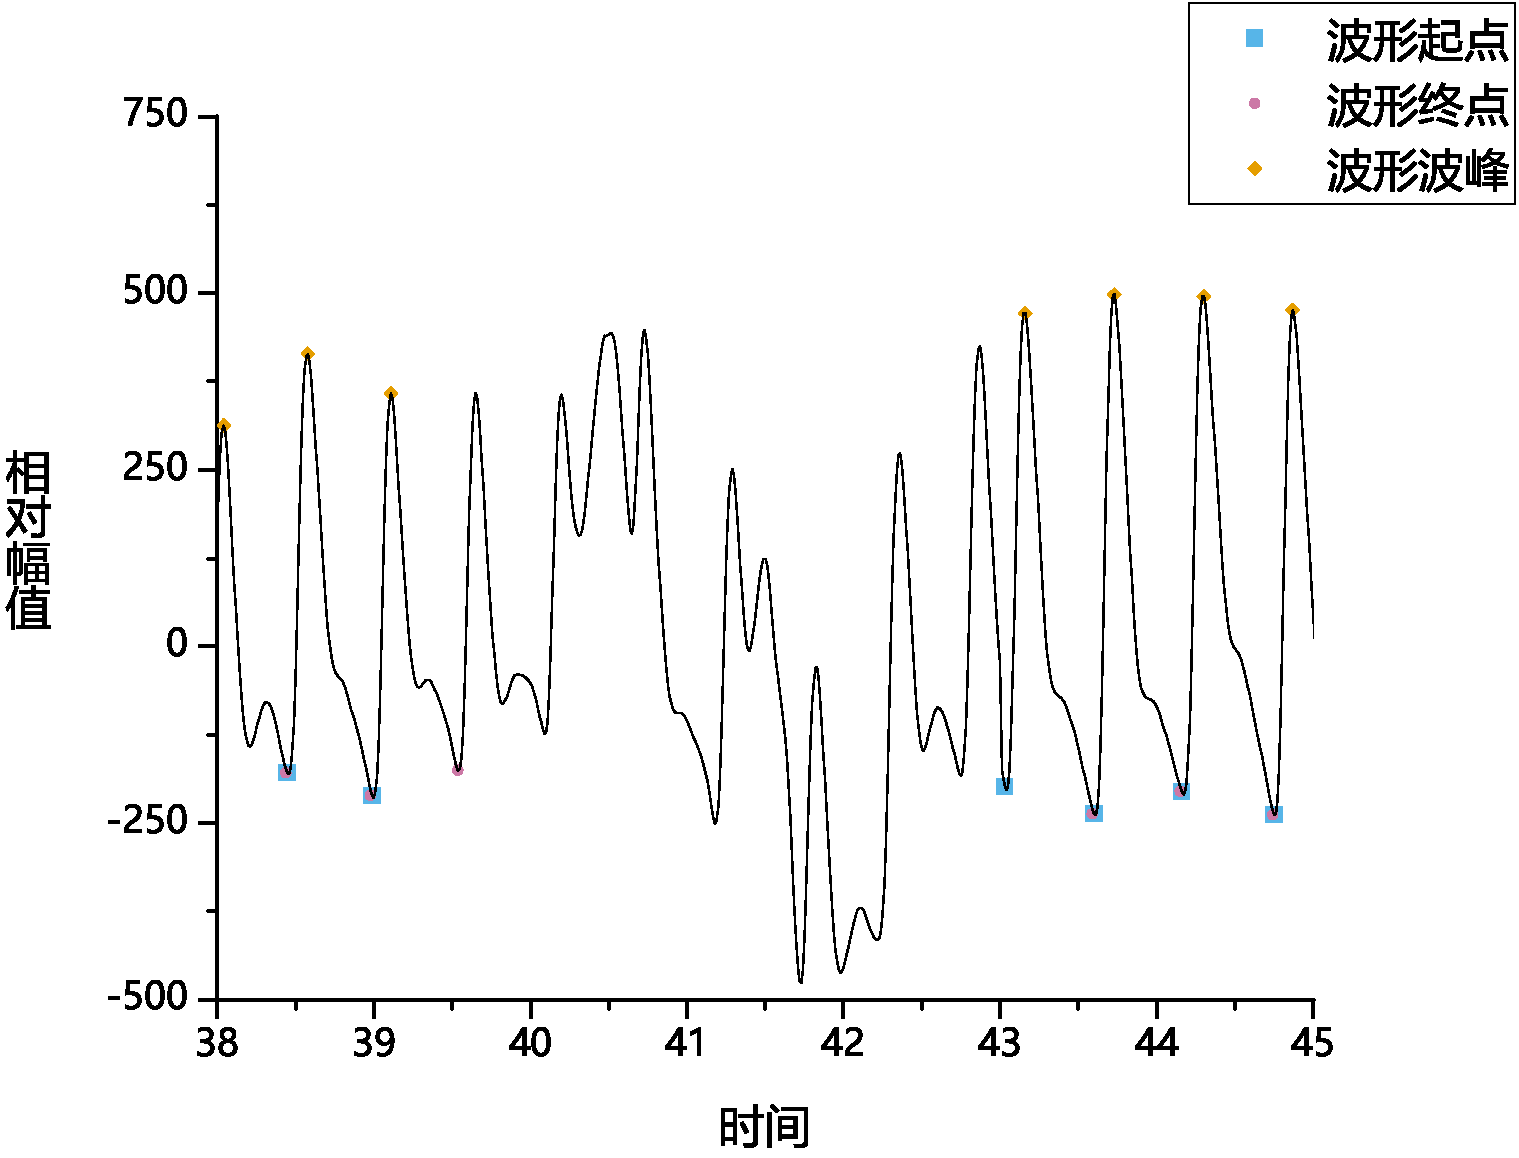
\includegraphics[width=7.5cm]{pulse_preprocess/check/why}
    }
    \quad
    \subfigure[\label{fig:c_xjh}被试XJH的波形检测结果(局部),6.5s处有明显错检]{
        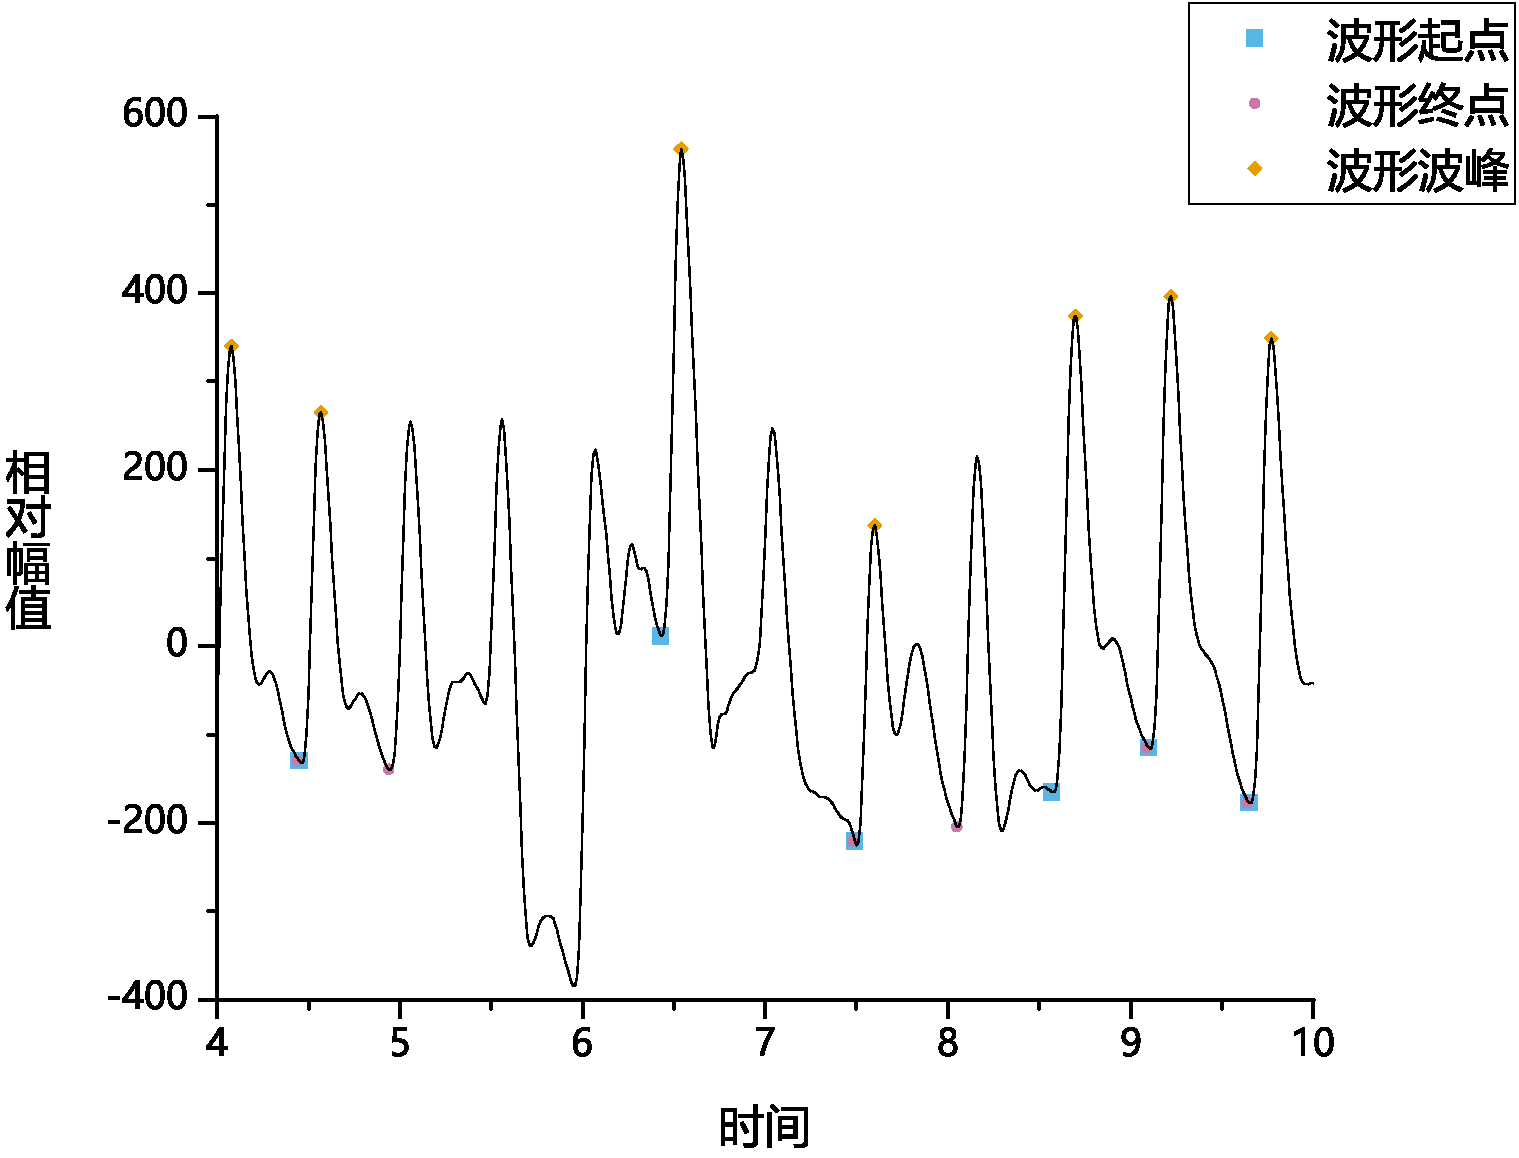
\includegraphics[width=7.5cm]{pulse_preprocess/check/xjh}
    }
    \caption{\label{fig:detect_details2}SCV算法对复杂信号的检测效果示意(补充)}
\end{figure}

\section{基于SCV检测算法的一个详尽实例}

基于\autoref{fig:samplesignal}中实采信号,SCV算法对其进行波形定位检测的初筛结果如\autoref{fig:detectcheck}所示,图中波峰处数字为该波形的初筛编号。
各复核标准及最终加权投票(权值参考\autoref{tab:voting})的输出如\autoref{tab:detect}所示,
其中,输出值为0代表该初筛波形被判定为正常波形,否则为干扰段。
\begin{figure}[htbp]
    \centering
    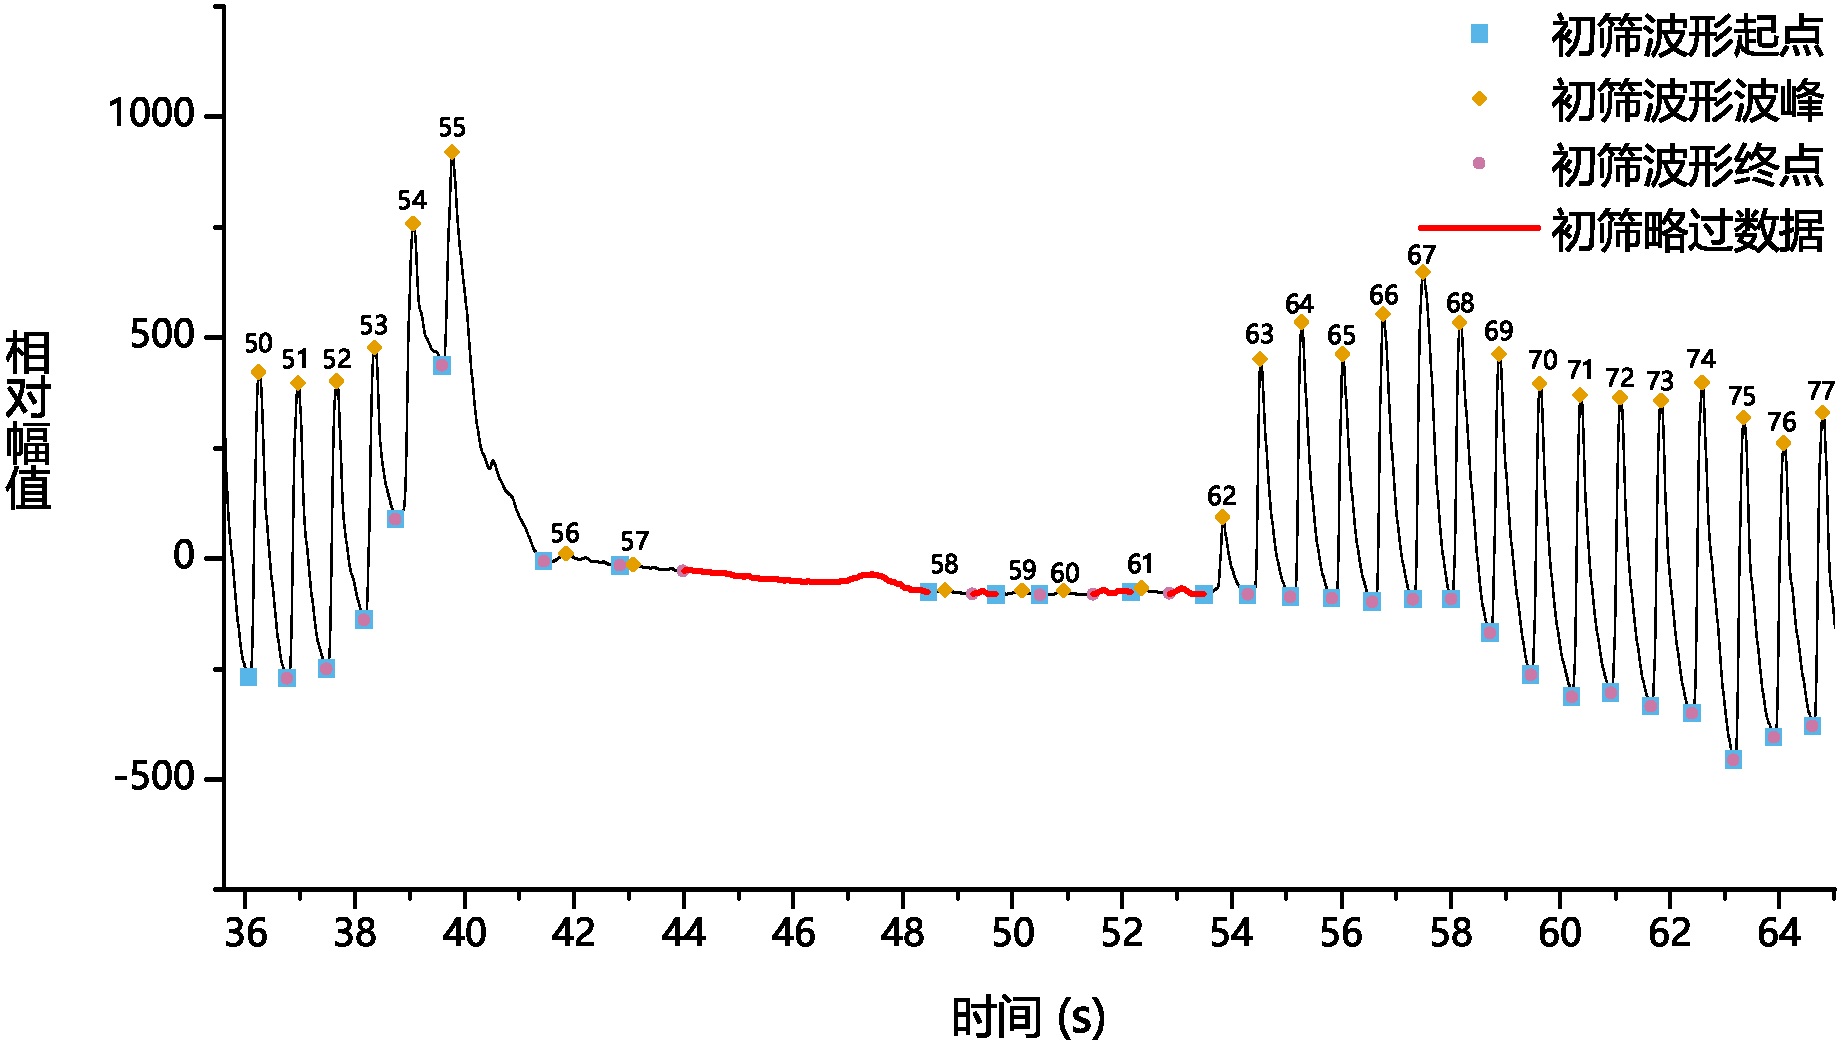
\includegraphics[width=0.9\linewidth]{pulse_preprocess/detectcheck}
    \caption{\label{fig:detectcheck}PPG波形检测算法初筛结果}
\end{figure}
\begin{table}[htbp]
    \centering
    \caption{\label{tab:detect}SCV算法对初筛波形的复核及决策输出(局部)}
    \begin{tabularx}{\linewidth}{X<{\centering}ccccX<{\centering}cX<{\centering}X<{\centering}}
    \toprule
    \multirow{2}[4]{*}{\textbf{波形编号}} & \multicolumn{3}{c}{\textbf{单项复核评估标准输出}} & \multicolumn{2}{c}{\textbf{绝对多数投票}} & \multicolumn{2}{c}{\textbf{加权投票}} & \multirow{2}[2]{*}{\textbf{人工裁定}}\\
    \cmidrule{2-8} & \textbf{功率} & \textbf{标准差} & \textbf{基线} & \textbf{输出} & \textbf{判定} & \textbf{输出} & \textbf{判定} \\
    \midrule
    ……    & ……    & ……    & ……    & ……    & ……    & ……    & …… & ……\\
    52    & 0     & 0     & 0     & 0     & 正常波形  & 0     & 正常波形 & 正常波形\\
    53    & 0     & 0     & 1     & 0     & 正常波形  & 0.2   & 正常波形 & 正常波形\\
    54    & 1     & 0     & 1     & 1     & 干扰段   & 0.6   & 干扰段 & 干扰段\\
    55    & 1     & 0     & 1     & 1     & 干扰段   & 0.6   & 干扰段 & 干扰段\\
    56    & 1     & 1     & 1     & 1     & 干扰段   & 1     & 干扰段 & 干扰段\\
    57    & 1     & 1     & 1     & 1     & 干扰段   & 1     & 干扰段 & 干扰段\\
    58    & 1     & 1     & 1     & 1     & 干扰段   & 1     & 干扰段 & 干扰段\\
    59    & 1     & 1     & 0     & 1     & 干扰段   & 0.8   & 干扰段 & 干扰段\\
    60    & 1     & 1     & 1     & 1     & 干扰段   & 1     & 干扰段 & 干扰段\\
    61    & 1     & 1     & 0     & 1     & 干扰段   & 0.8   & 干扰段 & 干扰段\\
    62    & 1     & 1     & 0     & 1     & 干扰段   & 0.8   & 干扰段 & 干扰段\\
    63    & 1     & 1     & 0     & 1     & 干扰段   & 0.8   & 干扰段 & 干扰段\\
    64    & 0     & 0     & 0     & 0     & 正常波形  & 0     & 正常波形 & 正常波形\\
    ……    & ……    & ……    & ……    & ……    & ……    & ……    & …… & ……\\
    80    & 1     & 0     & 0     & 0     & 正常波形  & 0.4   & 正常波形 & 正常波形\\
    ……    & ……    & ……    & ……    & ……    & ……    & ……    & …… & ……\\
    \bottomrule
    \end{tabularx}%
\end{table}%

\section{一个附录}
开发软件及工具

\section{批处理操作及参数设置说明}
一、目的

保存当前对PPG读取分析的相关操作,供下次调用快速使用。典型的应用场景为,调整了脉搏波的输出特征后,需要对所有数据进行新一轮的分析,此时脉搏波的定位结果可以完全沿用上一轮分析结果。若上一轮分析结果已被保存,则当前新一轮分析即可批量处理完成。

二、操作流程

1. 设置需要批处理的目录

批处理是以目录为单位进行。通过批处理->生成模板,选择目录后,即可在该目录下生成空白的配置文件。

2. 手动调整配置文件的相关参数

默认的配置文件具有的功能有限。需要根据具体数据灵活调整,由于一般数据文件在整个分析周期内是固定不变的。因此,配置文件设置完成后(特别是对脉搏波波形的取舍设置),可以在整个分析周期内通用。

3. 选择设置好的配置文件完成批处理

通过软件选择批处理->开始批处理,选择相应的配置文件,按配置完成批处理过程。

三、参数配置说明

1. 语法

配置文件必须是合法的Json文件。

2. 字段说明

\Rnum{1}. path 

当前需要批处理的目录。无需手动调整。

\Rnum{2}. PEstate

当前目录下所有数据的PE状态,值域[0,1]。需要手动设置。

\Rnum{3}. mode

当前批处理所需要进行的批处理操作,可自定义设置。目前支持打开文件、算法初步确认、人工手动调整检测结果、导出检测结果、开始特征分析、导出分析特征及分析结果上传等7种操作。其中,后6种文件操作在批处理过程中统一配置。分别通过mode的1位来完成控制。算法初步确认对应mode的最低位。mode的默认值为31,即0b011111,即对当前目录下所有数据文件进行出数据特征上传外的所有操作。
需要注意的是,可配置的6个操作有着逻辑上的依赖关系,某些配置可能会导致程序无法运行。如出现此种情况,请联系作者。

\Rnum{4}. files

当前批处理操作所需处理的所有数据文件项。批处理会依次对file中所有数据项进行处理。需要对其中的一定数据项进行自定义配置。

\Rnum{5}. path in files

需要处理的数据文件名。默认生成,无需修改。

\Rnum{6}. skipped in files

是否跳过处理该数据文件,可自定义配置。默认为false,即不跳过。

\Rnum{7}. pulses in files

对该数据波形自动分析结果得到的脉搏波波形的删除或新增操作,可自定义配置。默认为空,即接受算法全部处理结果。若需要配置,需要新增一个包含type与points两个字段的Json数据项至pulses。可根据需要配置多个这样的数据项。

\Rnum{8}. type in pulses in files

指定对脉搏波波形操作类型,必须配置。可选字段,A与R。前者对应新增(add),后者对应删除(remove)。目前不接受其他字段。

\Rnum{9}. Points in pulses in files

定义需要新增或移除的脉搏波的坐标位置,必须是三元数组(对应起点、峰值点及终点),必须配置。其中,峰值点数值决定了当前波形的新增或移除是否成功。新增波形时,三者的数值准确性要求较低,可允许10以内的误差。移除时,必须保证坐标位置的准确性。

四、配置范例及说明

\lstinputlisting[caption={配置范例},label=lst:json,style=myJava]{code/appendix/demo.json}

上述配置文件可对\path{D:/UrgeData/Documents/ppgdata/No}文件夹下的\path{by_wavePLETH_2017080113.csv}等文件进行批处理。其中,PEstate被设置为0,表示当前目录下全为健康人群数据文件。
mode被配置为31,所有文件会完成算法初步确认、人工手动调整检测结果、导出检测结果、开始特征分析、导出分析特征等操作。在对\path{by_wavePLETH_2017080113.csv}文件处理时,
不需跳过处理,对算法的自动检测结果需先移除$(91,105,177)$处的脉搏波波形,再在$(91,105,177)$处新增一个脉搏波波形。
}